\section{Le parseur et la sérialisation XMI}
\label{sec:parseur_XMI}

L'un des principaux objectifs de ce projet est de permettre la transformation d'un programme écrit en CHIPS vers une représentation XMI conforme au méta-modèle Ecore du langage. Cette étape constitue un élément essentiel de la chaîne de modélisation, puisqu'elle permet de convertir une description textuelle en un modèle structuré pouvant être manipulé par différents outils reposant sur les technologies de l'Eclipse Modeling Framework (EMF). La difficulté ne réside pas uniquement dans la lecture du langage mais également dans l'interprétation correcte de sa structure afin de reconstruire fidèlement les relations définies par le méta-modèle. \\

\RemarkBox
{Note terminologique}
{
Un méta-modèle est, par analogie, la "grammaire" d'un modèle. Dans le projet de CHIPS, il prend la forme de diagrammes de classes Ecore qui définissent de manière stricte les concepts du langage CHIPS (entités, attributs, relations). Le fichier chips1.1.ecore est donc le schéma directeur qui dicte comment un fichier XMI doit être structure pour être valide.
}

Pour atteindre cet objectif, plusieurs évolutions ont été apportées à l'infrastructure existante. Le parseur historique, développé avec Yacc/Bison et Flex, ne permettait pas de prendre en charge certaines constructions modernes du langage, notamment les templates du C++, qui sont utilisés pour définir les classes génériques lors de la compilation. Une réécriture basée sur ANTLR4 a donc été entreprise afin de disposer d'une représentation syntaxique plus robuste et mieux adaptée à l'interprétation du langage. Cette nouvelle architecture facilite également le parcours de l'arbre syntaxique abstrait, étape indispensable à la construction du modèle XMI. \\

Cette partie présente ainsi les différentes briques mises en œuvre pour réaliser cette transformation. Nous commencerons par décrire la migration vers ANTLR4 ainsi que la conception de la table des symboles utilisée lors de l'analyse du programme. Nous expliquerons ensuite comment le parcours de l'arbre syntaxique, réalisé au moyen du patron de conception visiteur, permet de construire progressivement le modèle correspondant. Enfin, nous détaillerons les adaptions apportées à la table des symboles afin de résoudre correctement les références entre les différents éléments du méta-modèle et de produire un fichier XMI valide. \\

Il y a deux tables des symboles distinctes à gérer (cf. figure \ref{fig:architecture_parseur_xmi}), celle du parseur et celle du générateur XMI. 
Etant donné que le méta-modèle, pour être respecté, implique que le parseur fasse bien plus que parser. Il doit 
surtout faire le contrôle de type car le langage est fortement typé, mais aussi des vérifications des portées des 
variables dans le programme CHIPS. \\

\begin{figure}
    \centering
    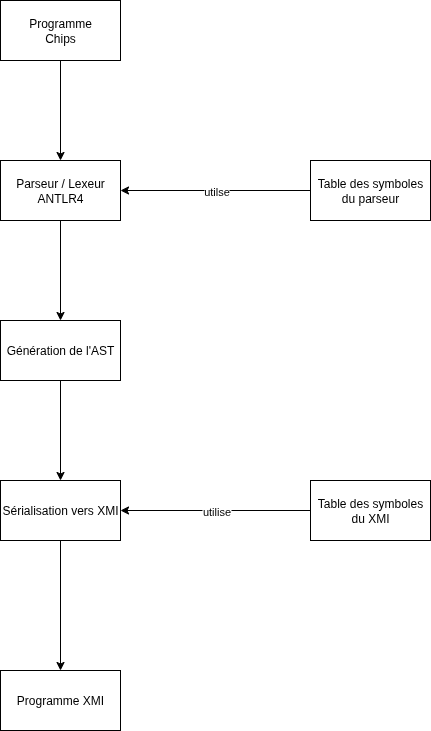
\includegraphics[width=0.3\textwidth]{images/architecture_parseur_xmi.png}
    \caption{Architecture du parseur et du générateur XMI}
    \label{fig:architecture_parseur_xmi}
\end{figure}


\subsection{Le parseur}
\label{sec:parseur}

Les premiers travaux consacrés au développement du langage CHIPS ont conduit à la réalisation d'un premier interpréteur reposant sur les outils Yacc/Bison et Flex. Cette architecture assurait l'analyse lexicale et syntaxique des programmes CHIPS afin de produire un arbre syntaxique abstrait représentant leur structure. Cet AST constituait ensuite le point d'entrée des différents traitements réalisés par l'interpréteur, notamment la génération d'un modèle XMI conforme au méta-modèle du langage. \\

Cette première implémentation a permis de démontrer la faisabilité de la chaîne d'interprétation du langage et de valider les principaux choix architecturaux retenus pour le projet. Elle constitue aujourd'hui encore la base sur laquelle reposent les développements réalisés pendant le stage. \\

Toutefois, l'évolution du langage CHIPS a progressivement fait apparaître de nouvelles exigences, notamment avec l'introduction des templates C++. Ces nouvelles constructions syntaxiques ont conduit à faire évoluer l'architecture de l'analyseur afin de conserver une grammaire claire et facilement extensible. Les sections suivantes présentent les principaux travaux réalisés dans cette optique. \\

\subsubsection{Migration vers ANTLR4}
\label{sec:migration_antlr4}

L'analyseur développé lors des travaux antérieurs reposait sur une grammaire écrite pour Yacc/Bison et Flex, 
permettant de reconnaître les différentes constructions du langage CHIPS et de construire l'arbre syntaxique 
abstrait correspondant. Cette architecture n'assurait pas fidèlement la compatibilité avec l'approche dirigée par les modèles, par conséquent 
pour augmenter cette fidélité de l'AST du parseur vis-à-vis du méta-modèle.

% Cette architecture répondait pleinement aux besoins du langage dans son état initial et 
% permettait de générer correctement l'ensemble des structures alors supportées. \\

Au cours du stage, l'apparition des templates C++, permettant de définir des classes génériques passant de 297 à 97 classes C++, a introduit une nouvelle problématique. Ces constructions possèdent une syntaxe fortement imbriquée qui rend leur prise en charge particulièrement complexe dans la grammaire Bison existante. Afin de permettre leur intégration tout en conservant les fonctionnalités déjà développées, le choix a été fait de migrer vers ANTLR4, dont les mécanismes d'analyse offrent une plus grande souplesse pour décrire ce type de structures syntaxiques. \\

Cette migration constitue la principale évolution de la chaîne d'analyse réalisée pendant ce stage. Elle a nécessité l'adaptation des différents traitements reposant sur l'AST généré par l'analyseur. \\

\subsubsection{La table des symboles pour le parseur}
\label{sec:table_symbole_parseur}

Il a fallu implémenter une table des symboles assez robuste pour qu'elle permette de ne pas instancier deux classes différentes qui auraient le même nom dans un programme CHIPS. La classe SymbolTable sert de registre central des noms visibles pendant l'analyse du programme. Son rôle est de mémoriser ce qui a été déclaré, avec son type logique, pour que le reste du parseur puisse retrouver rapidement une variable, une fonction, un channel, un objet ou un bloc sans ambiguïté. \\

\paragraph{Structure interne}

Elle repose sur plusieurs niveaux de stockage.
\begin{itemize}[label=$\bullet$]
    \item \texttt{scopes} contient une pile de scopes, chaque scope étant une table associant un nom à un symbole.
    \item chaque \texttt{Symbol} stocke trois choses : la valeur réelle dans un \texttt{std::any}, le nom, et la catégorie du symbole via \texttt{SymbolKind}.
    \item en plus de ça, il y a deux tables séparées pour les sorties de fonctions et les paramètres de fonctions.
    \item enfin, \texttt{declarated\_block\_system} garde le type associé à certains blocs déclarés.
\end{itemize}

L'idée générale est donc : un stockage principal pour les symboles ordinaires, et des structures annexes pour les cas particuliers liés aux fonctions et aux blocs. \\

\RemarkBox
{Points important}
{
    CHIPS est un langage qui définit des modèles sous la forme de blocs fonctionnels pour représenter un processus, 
    en les connectant entre eux, on permet au modèle de réaliser une suite d'opérations.
}

\paragraph{Méthodes principales}

Les méthodes les plus importantes sont assez simples à lire.

\begin{itemize}
    \item \texttt{enterScope()} et \texttt{exitScope()} ouvrent et ferment un scope.
    \item \texttt{declare...()} enregistre un symbole d'un certain genre : variable, variable contextuelle, channel, fonction, objet, bloc\dots
    \item \texttt{lookup...()} recherche un symbole dans les scopes, en partant du plus interne vers le plus externe.
    \item \texttt{declareFunctionOutput()} et \texttt{declareFunctionParameter()} gèrent les métadonnées des fonctions.
    \item \texttt{declareBlock()} et \texttt{getTypeOfDeclaratedBlock()} servent à mémoriser puis relire le type d'un bloc.
    \item \texttt{dump()} affiche un état lisible de la table pour le débogage.
\end{itemize}

\paragraph{Exemple d'utilisation}

En pratique, l'utilisation de ces fonctions se réalise dans cet ordre :

\begin{lstlisting}[caption={Exemple d'utilisation de SymbolTable}]
    auto& table = chips::SymbolTable::getInstance();
    table.enterScope();
    table.declareVariable("x", someValue);
    // dom somethings
    if(table.lookupVariable("x").has_value()){
        // do somethings
    }else{
        // handle error
    }
    table.exitScope();
\end{lstlisting}
Ici, on entre dans un scope, on va déclarer une variable ayant pour identifiant "x". On va effectuer un certain nombre d'opérations, puis on va chercher à retrouver la variable "x" dans la table des symboles. Si elle est trouvée, on peut l'utiliser et effectuer des opérations dessus. Sinon, on gère l'erreur de manière appropriée. Enfin, on quitte le scope, ce qui supprime toutes les variables déclarées dans ce scope de la table des symboles.



\subsection{Sérialisation vers XMI}
\label{sec:XMI}

Les travaux antérieurs ont également permis de développer une première chaîne de transformation capable de convertir un programme CHIPS en un modèle XMI conforme au méta-modèle Ecore. Cette étape constitue le coeur de l'interprétation du langage puisqu'elle permet de transformer une représentation textuelle en un modèle exploitable par les différents outils de l'ingénierie dirigée par les modèles. Cette première architecture reposait sur un parcours de l'arbre syntaxique abstrait afin de générer progressivement les différents éléments du document XMI. \\

Cette première implémentation a permis de démontrer la faisabilité de la sérialisation du langage et de mettre en place les principaux mécanismes nécessaires à la génération des modèles. Elle introduisait notamment un visiteur chargé du parcours de l'AST ainsi qu'une première table des symboles permettant de résoudre les références présentes dans le modèle généré. \\

L'évolution de l'interpréteur réalisée au cours du stage a toutefois nécessité de faire évoluer cette architecture (cf. figure \ref{fig:architecture_parseur_xmi}) afin de l'adapter au nouvel AST produit par ANTLR4 tout en conservant les principes de fonctionnement établis par les travaux antérieurs. \\

\subsubsection{Evolution du visiteur de génération du XMI}
\label{sec:generation_XMI}

Les premiers travaux de sérialisation reposaient sur un visiteur chargé de parcourir récursivement l'arbre syntaxique abstrait afin de construire progressivement le modèle XMI correspondant. Chaque méthode de visite avait pour rôle de traduire un type de noeud particulier en son équivalent dans le méta-modèle Ecore tout en assurant la cohérence de la structure produite. \\

Le principe général de cette architecture a été conservé au cours du stage. En revanche, la migration vers ANTLR4 ainsi que l'évolution du langage CHIPS ont nécessité de faire évoluer plusieurs mécanismes internes du visiteur afin de prendre en compte la nouvelle organisation de l'AST et les nouvelles constructions syntaxiques introduites. \\

Les développements réalisés ont principalement porté sur la restructuration du visiteur, la factorisation de traits communs et l'amélioration de la génération des différents éléments du modèle XMI. \\

\subsubsection{La table des symbôles pour le XMI}
\label{sec:table_symbole_XMI}

La génération d'un modèle XMI nécessite de retrouver précisément les différents éléments déclarés dans un programme afin de construire correctement les références imposées par le méta-modèle Ecore. Les travaux antérieurs répondaient à cette problématique au moyen d'une première table des symboles associant les identifiants rencontrés lors du parcours de l'AST aux chemins XMI des éléments correspondants. \\ % citer rapport projet

Cette première architecture répondait aux besoins de la chaîne de transformation initiale mais devait évoluer afin d'accompagner les modifications apportées au nouvel AST ainsi que les nouvelles fonctionnalités du langage. Les mécanismes de résolution des références ont notamment été généralisés afin de prendre en compte davantage de catégories de symboles et de centraliser les informations nécessaires à la génération du modèle. \\

Les travaux réalisés au cours du stage ont ainsi conduit à une refonte de cette structure de données afin d'en faire un composant central de la sérialisation XMI. Cette évolution améliore la robustesse du processus de génération, facilite la résolution des références entre les différents éléments du modèle et prépare l'infrastructure aux futures évolutions du langage CHIPS. \\

\FloatBarrier

\newpage